
\chapter{m-ary increasing trees}
% LTeX: language=de-DE
In diesem Kapitel werden die Teilmenge der \textit{linear preferential attachment trees}, mit Parametern der Form $\chi < 0$ und $\rho > 0$ näher betrachtet. Wie schon im ersten Kapitel bemerkt, ändert die Normierung von allen Gewichten $w_k$ mit einer Konstante $c \in \mathbb{R}$ nicht die Verteilung der Bäume. Infolgedessen, betrachten wir $\chi = -1$ und prüfen, bei welchen $\rho \in \mathbb{R}^{+}$ es zu negative Gewichten kommt.\\
Für $\chi = -1$ sind die Gewichte der \textit{linear preferential trees} durch 
\[
    w_k = \chi k + \rho =  \rho - k 
\]
festgelegt. Für $k > \rho$ folgt daraus, dass $w_k < 0$. Daher ist die einzige Möglichkeit negative Gewichte zu vermeiden, $w_m = 0$, für ein $m \in \mathbb{N}$ sicherzustellen. In diesem Fall kann einem Knoten mit $m$ Kindern kein weiterer Knoten hinzugefügt werden, und die weiteren Gewichte $w_n, n > m$ sind von keiner Relevanz. Auf $\rho$ bezogen, heißt das, dass $\rho = m\in \mathbb{N}$, falls $\chi = -1$, bzw. $\rho= m\chi, m \in \mathbb{N}$, falls wir $\chi$ nicht zu $-1$ normieren.\\
Bis jetzt wurden Bäume nur in einer ungeordneten Weise betrachtet, d.h. es zählte nur welche Geschwister ein Knoten hat, und nicht die Reihenfolge der Geschwister. Da in dieser Teilmenge der \textit{linear preferential attachment trees} die Anzahl der Kinder pro Knoten durch $m$ beschränkt ist, können wir die Bäume auch in einer geordneten Weise interpretieren. Das Beispiel $T_n^{-1,2}$ illustriert wie wir diesen Gedanken nachverfolgen können.
\begin{Beispiel}
    Die Gewichte von einem Knoten $v$ in einem $T_n^{-1,2}$ haben die Form: 
    \[
        w_k = 2 - k, k \in \{0,1,2\},
    \]
    wobei $k$ der Ausgangsgrad von $v$ ist. Wir können die Gewichte umschreiben, indem wir die Gewichte proportional zu den externen Kindern von $v$ auffassen. Es gibt $e = m - k = 2-k$ externe Kinder $e$ von einem Knoten $v$ und somit haben die Gewichte die Form 
    \[
        w_k = 2 -k = 2 - (2-e) = e, e \in \{0,1,2\}. 
    \]
    Das bedeutet jeder Knoten hat Gewicht direkt proportional zu der Anzahl der externen Knoten. Diese Eigenschaft erlaubt uns den Aufbau von $T_n^{-1,2}$ geordnet zu interpretieren. Dazu beginne man mit einem vollständigen unendlichen 2-ären Baum, mit Kindern von einem Knoten mit $\{1,2\}$ beschriftet und dann zufällig Uniform permutiert. Wir konstruieren dann den $(T_n^{-1,2})_{n \in \mathbb{N}}$ innerhalb von diesem $\mathcal{T}_2$ Baum: in jedem Schritt wird ein externer Knoten von $T_n^{-1,2}$ mit Beschriftung aus $\mathcal{T}_2$ uniform ausgewählt und hinzugefügt (Siehe Abbildung \ref{picture binary trees})
\end{Beispiel}

\usetikzlibrary{shapes.geometric}
\begin{figure}[h!]
\begin{center}
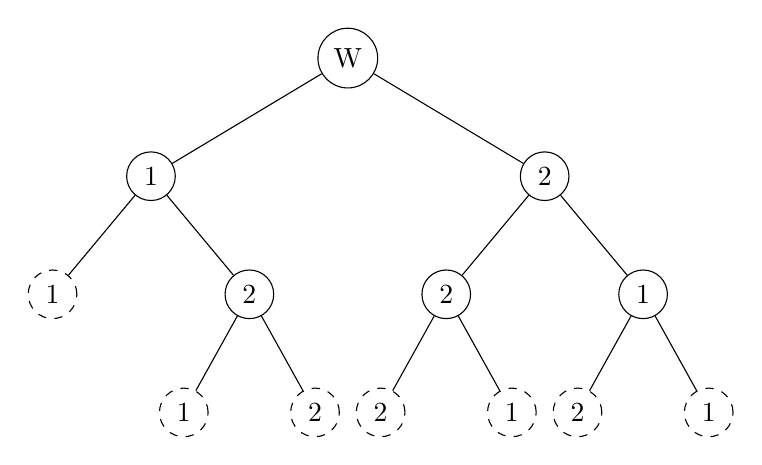
\begin{tikzpicture}[level/.style={sibling distance=50mm/#1}]
	

	\node[circle,draw] {W}
		child {node[circle,draw] {1}
			child {node[circle,draw,dashed]  {1}}
            child {node[circle,draw]  {2}
                child{node[circle,draw,dashed]{1}}
                child{node[circle,draw,dashed]{2}}}}
		child {node[circle,draw] {2}
			child {node[circle,draw]  {2}
                child{node[circle,draw,dashed]{2}}
                child{node[circle,draw,dashed]{1}}}
            child {node[circle,draw]  {1}
                child{node[circle,draw,dashed]{2}}
                child{node[circle,draw,dashed]{1}}}
		};
\end{tikzpicture}
\caption{\label{picture binary trees}Beispiel für eine Konstruktion von einem $T_n^{-1,2}$ Baum. Die externen Knoten sind mit gestrichelter Linien abgebildet und $W$ ist die Wurzel}.
\end{center}
\end{figure}
Die geordnete Interpretation von $T_n^{-1,2}$ entspricht daher einem zufälligen Binärsuchbaum. Diese sind aber einer der elementaren Beispiele von Split Bäumen behandelt in \cite{devroye1998universal}, welche durch den Split Vektor $\mathcal{P} = (U,1-U)$ und $U \sim Uniform[0,1]$ charakterisiert ist. Dies steht nicht in Widerspruch zu Satz \ref{main theorem paper}, denn obwohl die Bäume $T_n^{-1,2}$ und $T_n^{(U,1-U)}$ in der ungeordneten Interpretation dieselbe Verteilung haben, ist die Verteilung von $T_n^{\mathcal{P}}$ nicht eindeutig durch $\mathcal{P}$ festgelegt. Der Split Vektor $\mathcal{P}$ ist nach Bemerkung \ref{Bemerkung PD Verteilungen} nur bis auf (zufällige) Permutationen eindeutig, bedeutet es muss eine (zufällige) Permutation von $\mathcal{P}^1 := (P_1,1-P_1) \sim GEM(-1,2)$ geben, sodass $\mathcal{P}^1 \stackrel{\mathcal{L}}{=} \mathcal{P}^2 := (U,1-U)$. Nach Satz \ref{Main theorem CRP} ist $P_1 \sim \beta(1,2)$ und hat somit nach Definition \ref{definition beta distribution} Wahrscheinlichkeitsdichte $2x$ und $1-P_1$ hat Dichte $2-2x$. Falls wir annehmen, dass die Permutation unabhängig von $(P_1,1-P_1)$ ist, so kann man der Permutation Wahrscheinlichkeiten zuordnen, sodass $(P_1,1-P_1)$ mit Wahrscheinlichkeit $p_1$ und $(1-P_1,P_1)$ mit Wahrscheinlichkeit $p_2$ gewählt wird. Wir versuchen dann $p_1,p_2$ zu bestimmen, sodass wir die Verteilung $(U,1-U)$ zurückgewinnen. Wir definieren unsere zufällige Permutation mit $(\tilde{P}_1,\tilde{P}_2)$ und berechnen für $a \in [0,1]$
\begin{align*}
 \mathbb{P}(\tilde{P}_1 \leq a) &=  \mathbb{P}(P_1 \leq a| \tilde{P}_1 = P_1)\mathbb{P}(\tilde{P}_1 = P_1) + \mathbb{P}(P_1 \leq a| \tilde{P}_1 = P_2)\mathbb{P}(\tilde{P}_1 = P_2) \\
&= \mathbb{P}(P_1 \leq a| \tilde{P}_1 = P_1)p_1 + \mathbb{P}(P_1 \leq a| \tilde{P}_1 = P_2)p_2 \\
&= \int_{0}^{a}p_12x \textnormal{dx} + \int_{0}^{a}p_2(2-2x) \textnormal{dx}\\
&= \int_{0}^{a}p_12x + p_2(2-2x) \textnormal{dx}.
\end{align*}
Somit hat $\tilde{P}$ Wahrscheinlichkeitsdichte $p_12x + p_2(2-2x)$.
$U$ hat nach Voraussetzung Wahrscheinlichkeitsdichte $1$ und mit einem Koeffizientenvergleich erkennt man sofort, dass $p_1 = p_2 = \frac{1}{2}$ sein muss, damit die Dichten Übereinstimmen. In anderen Worten stimmt die Verteilung von $(P_1,1-P_1) \sim GEM(-1,2)$ nach einer uniformen Permutation mit $(U,1-U)$ überein. Da $(P_1,P_2) \sim PD(-1,2)$ eine  absteigende Anordnung von $(P_1,P_2) \sim GEM(-1,2)$ (nach Definition \ref{GEM und PD Verteilungen}), ist $PD(-1,2)$ eine absteigende Anordnung und somit eine Permutation von $(U,1-U)$. Falls wir $(P_1,1-P_1) \sim PD(-1,2)$ definieren, können wir die Verteilung von $P_1$ mit $a \in [0,1]$ bestimmen 
\begin{align*}
    \mathbb{P}(max(U,1-U) \leq a) &= \mathbb{P}(U \leq a \cap 1-U \geq a)\\
    = \mathbb{P}(1-a \leq U \leq a) &= \mathbb{P}(U \leq 2a - 1)\\
    &= \begin{cases}
        0 & a < 0.5 \\
      2a-1  & 0.5\leq a\leq 1\\
      1 & 1  > a 
    \end{cases}
\end{align*}
und somit ist $PD(-1,2) \stackrel{\mathcal{L}}{=} U(\frac{1}{2},1)$. \\

Die Betrachtungsweise von $T_n^{-1,m}$, als geordnete Bäume lässt sich auch auf $m > 2$ verallgemeinern. Diesmal betrachten vollständige $\mathcal{T}_m$ Bäume, mit Kindern von einem Knoten mit $\{1,...,m\}$ beschriftet und dann zufällig Uniform permutiert, wieder wird $(T_n^{-1,m})_{n \in \mathbb{N}}$ in $\mathcal{T}_m$ eingebettet und in jedem Schritt ein externer Knoten von $(T_n^{-1,m})_{n \in \mathbb{N}}$ mit Beschriftung in $\mathcal{T}_m$ uniform ausgewählt und hinzugefügt. Diese geordnete Konstruktion von einem Baum wird mit \textit{m-ary increasing tree} bezeichnet. Wir bestimmen jetzt den Split Vektor welcher den \textit{m-ary increasing tree} auch für $m >2$ charakterisiert.
\begin{theorem}
    \label{Satz mary increasing trees}
    Sei $m \geq 2$. Die Folge von \textit{linear preferential attachment trees} $(T_n^{-1,m})_{n \in \mathbb{N}}$, betrachtet als m-ary increasing Trees haben dieselbe Verteilung wie die Folge der Split Bäume $(T^\mathcal{P}_n)_{n \in \mathcal{N}}$, mit 
    \[
    \mathcal{P} = (P_i)_{i \in \mathbb{N}} \sim Dir(\frac{1}{m-1},...,\frac{1}{m-1}),
    \]
    wobei mit $Dir$ die Dirichlet-Verteilung gemeint ist.
\end{theorem}

\begin{Definition}\textnormal{Dirichlet-Verteilung}\\
    Ein Wahrscheinlichkeitsvektor $(X_1,...,X_m)$ ($\sum_{i=1}^{m} X_i \geq 0$ und $X_i \geq 0$) der Länge $m$ ist $Dir(\alpha_1,...,\alpha_m)$ verteilt, falls die Wahrscheinlichkeitsdichte durch
    \[
    f(x_1,...,x_m) = \frac{\Gamma(\sum_{i=1}^{m}x_i)}{\prod_{i=1}^{m}\Gamma(x_i)} \prod_{i=1}^{m}x_i^{\alpha_i-1}
    \] 
    für $x_i \geq 0$ und $\sum_{i=1}^{m}x_i = 1$ und für sonstige $(x_1,...,x_m)$ durch $0$ gegeben ist.
\end{Definition}
\begin{proof}[Beweis von Satz \ref{Satz mary increasing trees}]
    
\end{proof}
